\documentclass[a4paper,10pt]{article}
\usepackage[utf8]{inputenc}
\usepackage[american,danish,english]{babel}
\usepackage[T1]{fontenc}
\usepackage{pgfplots}
\usepackage{graphicx}
\usepackage{slashed}
\usepackage{amsmath, amssymb}
\usepackage{mathrsfs}
\usepackage{amsthm}
\usepackage{xcolor}
\usepackage{dsfont}
\usepackage{gensymb}
\usepackage{url}
\usepackage{lmodern}
\usepackage{subfigure}
\usepackage{ifthen}
\usepackage{gensymb}
\usepackage{booktabs}
\usepackage{multirow}
\usepackage{mathtools}
\usepackage{bm}
\usepackage{physics}
\usepackage[top=1in, bottom=1.25in, left=1in, right=1.25in]{geometry}
\renewcommand\[{\begin{equation*}} 
\renewcommand\]{\end{equation*}} 
\newcommand{\be}{\begin{equation}} 
\newcommand{\ee}{\end{equation}} 
\numberwithin{equation}{section}
\newcommand{\ot}{\:\otimes\:}
\newcommand{\Erf}{\:\text{Erf}}
\newcommand{\opl}{\:\oplus\:}
\newcommand{\ham}{\mathcal{H}}
\newcommand{\spin}{\mathscr{S}}
\newcommand{\dis}{\mathcal{D}}
\newcommand{\D}{\mathscr{D}}
\newcommand{\lp}{\left}
\newcommand{\rp}{\right}
\newcommand{\kbk}[3]{\ket{#1}\hspace*{-0.12cm}\braket{#2}{#3}} 
\DeclareMathOperator\atanh{atanh}
\usepackage[UKenglish]{isodate}
\usepackage{tikz}
\usetikzlibrary{decorations.pathmorphing}
\usetikzlibrary{arrows}
\newcommand{\midarrow}{\tikz \draw[-triangle 90] (0,0) -- +(.1,0);}
\tikzset{snake it/.style={decorate, decoration=snake}}
\usepackage[compat=1.1.0]{tikz-feynman}
\setcounter{section}{1}
\usepackage{float}
\usetikzlibrary{arrows,chains,matrix,positioning,scopes}
\usetikzlibrary{decorations.pathreplacing}
%\setcounter{secnumdepth}{0}
%nummerere alle equations atomatisk
\selectlanguage{english}
\date{\today}
\begin{document}
\selectlanguage{english}
\title{\textbf{Hand-in 1: String Theory 232}}
\author{Taro Valentin Brown }
\maketitle
\section*{Problem 1}
In this problem we are asked to calculate the central charge in the Virasoro algebra for $X^\mu$ from
\begin{equation} \label{eq:1}
    [L_m, L_{-m}]\ket{0;0}=L_m\left(L_{-m}\ket{0;0}\right)-L_{-m}\left(L_{m}\ket{0;0}\right)
\end{equation}
The reason we are able to uptain the central charge from this, is that for free bosons the Virasoro algebra should satisfy (eq. 2.6.19)
\begin{equation} \label{eq:2}
    [L_m, L_{n}]=(m-n)L_{m+n}+\frac{c}{12}(m^3-m)
\end{equation}
We will further make use of the fact that the definition of the generators is
\begin{equation}
    L_m=\frac{1}{2}\sum_{n=-\infty}^{\infty}:
    \alpha^{\mu}_{m-n}\alpha_{n\,\mu}:
\end{equation}
with 
\begin{equation}
    L_0=\frac{\alpha 'p^2}{4}+\sum_{n=1}^{\infty}\alpha_{-n} \alpha_n
\end{equation}
we note that since applying this to the ground state with zero momentum one finds,
\begin{equation} \label{eq:3}
\begin{aligned}
   L_0\ket{0;0}&= \left(\frac{\alpha 'p^2}{4}+\sum_{n=1}^{\infty}\alpha_{-n} \alpha_n\right)\ket{0;0}\\
   &=\frac{\alpha 'p^2}{4}\ket{0;0}+\sum_{n=1}^{\infty}\alpha_{-n} \alpha_n\ket{0;0}\\
   &=0
\end{aligned}
\end{equation}
which means that applying \eqref{eq:2} on $\ket{0;0}$ for the case of $m=-n$ simply gives
\begin{equation}\label{eq:algebra}
    [L_m, L_{-m}]\ket{0;0}=\frac{c}{12}(m^3-m)\ket{0;0}
\end{equation}
Further, let us recall the commutation relation for the nodes
\begin{equation} \label{eq:comm}
    [\alpha_m^\mu,\alpha^\nu_n]=m\eta^{\mu\nu}\delta_{m\,(-n
)}
\end{equation}
Now, let us treat the cases $m=\leq-1$, $m=0$, and $m\geq1$ for equation \eqref{eq:1} separately. First taking $m=0$ one finds
\begin{equation}
     [L_0, L_{0}]\ket{0;0}=(L_0^2-L_{0}^2)\ket{0;0}=0
\end{equation}
In the case of postive $m$ we can restrict the calculation even further because of the Virasoro algebra $2L_0=[L_1,L_{-1}]$ and equation \eqref{eq:3} leading to
\begin{equation}
     [L_{1}, L_{-1}]\ket{0;0}=2L_0\ket{0;0}=0
\end{equation}
Hence the first non-trivial case is for $m>1$:
\begin{equation} \label{eq:4}
    \begin{aligned}
       [L_{m}, L_{-m}]\ket{0;0}&=\frac{1}{4}\sum^{\infty}_{n=-\infty}\sum_{k=-\infty}^{\infty}\left[
       \left(
       \alpha_{m-n}\cdot \alpha_n
       \right)
       \left(
       \alpha_{-m-k}\cdot \alpha_k
       \right)
       -
       \left(
       \alpha_{-m-k}\cdot \alpha_k
       \right)
       \left(
       \alpha_{m-n}\cdot \alpha_n
       \right)
       \right]\ket{0;0}
    \end{aligned}
\end{equation}
We now use the fact that (Pol. eq 1.3.27b) for the ground state
\begin{equation}
    \alpha_m^i\ket{0;k}=0,~~\forall ~m>0
\end{equation}
Looking at the last term in the sum \eqref{eq:4}, we see that the state is annihilated either by the $\alpha_n$ or $\alpha_{m-n}$. We thus have
\begin{equation} \label{eq:4}
    \begin{aligned}
       [L_{m}, L_{-m}]\ket{0;0}&=\frac{1}{4}\sum^{\infty}_{n=-\infty}\sum_{k=-\infty}^{\infty}
       \left(
       \alpha_{m-n}\cdot \alpha_n
       \right)
       \left(
       \alpha_{-m-k}\cdot \alpha_k
       \right)
       \ket{0;0}\\
       &=\frac{1}{4}\sum^{\infty}_{n=-\infty}\sum_{k=-\infty}^{-1}
       \left(
       \alpha_{m-n}\cdot \alpha_n
       \right)
       \left(
       \alpha_{-m-k}\cdot \alpha_k
       \right)
       \ket{0;0}\\
       &=\frac{1}{4}\sum^{\infty}_{n=-\infty}\sum_{k=-m+1}^{-1}
       \left(
       \alpha_{m-n}\cdot \alpha_n
       \right)
       \left(
       \alpha_{-m-k}\cdot \alpha_k
       \right)
       \ket{0;0}
    \end{aligned}
\end{equation}
where we in the second line have employed the fact that $\alpha_k$ will annihilate the state for all $k>-1$ and in the third line used the fact $\alpha_{-m-k}$ will annihilate the state unless $k>-m$. Finally, using \eqref{eq:comm} we can commute the $\alpha$'s to the left through the $\alpha$'s on the right. The calculation is somewhat tedious to follow:
\begin{equation} \label{eq:4}
    \begin{aligned}
       [L_{m}, L_{-m}]\ket{0;0}
       =&\frac{1}{4}\sum^{\infty}_{n=-\infty}\sum_{k=-m+1}^{-1}
       \left(
       \alpha_{m-n}\cdot \alpha_n
       \right)
       \left(
       \alpha_{-m-k}\cdot \alpha_k
       \right)
       \ket{0;0}\\
       =&\frac{1}{4}\sum^{\infty}_{n=-\infty}\sum_{k=-m+1}^{-1}
       \alpha_{m-n}^\mu \alpha_{n\,\mu}\, 
       \alpha_{-m-k}^\nu\, \alpha_{k\,\nu}
       \ket{0;0}
       \\
       =&\frac{1}{4}\sum^{\infty}_{n=-\infty}\sum_{k=-m+1}^{-1}
       \alpha_{m-n}^\mu \left(
       \alpha_{-m-k}^\nu\alpha_{n\,\mu}+n\delta^{\nu}_{\mu}\delta_{n\,(m+k)} \right)\, \alpha_{k\,\nu}
       \ket{0;0}
        \\
       =&\frac{1}{4}\sum^{\infty}_{n=-\infty}\sum_{k=-m+1}^{-1}
       \alpha_{m-n}^\mu 
       \alpha_{-m-k}^\nu\alpha_{n\,\mu} \, \alpha_{k\,\nu}\ket{0;0}
       \\
       &+\frac{1}{4}\sum^{\infty}_{n=-\infty}\sum_{k=-m+1}^{-1} n\delta^{\nu}_{\mu}\delta_{n\,(m+k)}
       \alpha_{m-n}^\mu 
        \alpha_{k\,\nu}
       \ket{0;0}
        \\
       =&\frac{1}{4}\sum^{\infty}_{n=-\infty}\sum_{k=-m+1}^{-1}
       \alpha_{m-n}^\mu 
       \alpha_{-m-k}^\nu\left( \alpha_{k\,\nu}\alpha_{n\,\mu}+n\eta_{\mu\nu}\delta_{n,-k}\right)\ket{0;0}
       \\
       &+\frac{1}{4}\sum^{\infty}_{n=-\infty}\sum_{k=-m+1}^{-1} n\delta^{\nu}_{\mu}\delta_{n\,(m+k)}
     \left(
        \alpha_{k\,\nu} \alpha_{m-n}^\mu 
        +(m-n)\delta^{\mu}_{\nu}\delta_{n-m\,k}
     \right)
       \ket{0;0}
        \\
       =&\frac{1}{4}\sum^{\infty}_{n=-\infty}\sum_{k=-m+1}^{-1}
       \alpha_{m-n}^\mu 
       \alpha_{-m-k}^\nu \alpha_{k\,\nu}\alpha_{n\,\mu}\ket{0;0}
       \\
       &+\frac{1}{4}\sum^{\infty}_{n=-\infty}\sum_{k=-m+1}^{-1}
       n\eta_{\mu\nu}\delta_{n,-k} \alpha_{m-n}^\mu 
       \alpha_{-m-k}^\nu \ket{0;0}\\
       &+\frac{1}{4}\sum^{\infty}_{n=-\infty}\sum_{k=-m+1}^{-1} n\delta^{\nu}_{\mu}\delta_{n\,(m+k)}
        \alpha_{k\,\nu} \alpha_{m-n}^\mu 
       \ket{0;0}
       \\
       &+\frac{1}{4}\sum^{\infty}_{n=-\infty}\sum_{k=-m+1}^{-1} n(m-n)\delta^{\nu}_{\mu} \delta^{\mu}_{\nu}\delta_{n\,(m+k)}
       \ket{0;0}
    \end{aligned}
\end{equation}

\begin{equation} \label{eq:4}
    \begin{aligned}
       [L_{m}, L_{-m}]\ket{0;0}
       =&\frac{1}{4}\sum^{\infty}_{n=-\infty}\sum_{k=-m+1}^{-1}
      (\alpha_{-m-k}^\nu \alpha_{m-n}^\mu 
       +(m-n)\eta^{\mu\nu}\delta_{(m-n)\,(m+k)}) \alpha_{k\,\nu}\alpha_{n\,\mu}\ket{0;0}
       \\
       &+\frac{1}{4}\sum^{\infty}_{n=-\infty}\sum_{k=-m+1}^{-1}
       n\eta_{\mu\nu}\delta_{n,-k} (\alpha_{-m-k}^\nu \alpha_{m-n}^\mu 
       +(m-n)\eta^{\mu\nu}\delta_{(m-n)\,(m+k)})\ket{0;0}\\
       &+\frac{1}{4}\sum^{\infty}_{n=-\infty}\sum_{k=-m+1}^{-1} n\delta^{\nu}_{\mu}\delta_{n\,(m+k)}
        \alpha_{k\,\nu} \alpha_{m-n}^\mu 
       \ket{0;0}
       \\
       &+\frac{1}{4}\sum^{\infty}_{n=-\infty}\sum_{k=-m+1}^{-1} n(m-n)\delta^{\nu}_{\mu} \delta^{\mu}_{\nu}\delta_{n\,(m+k)}
       \ket{0;0}\\
=
&\frac{1}{4}\sum^{\infty}_{n=-\infty}\sum_{k=-m+1}^{-1}
\left(n(m-n)\eta^{\mu\nu}\eta_{\mu\nu}\delta_{n,-k}+n(m-n)\delta^{\nu}_{\mu} \delta^{\mu}_{\nu}\delta_{n\,(m+k)}\right) \ket{0;0}
    \end{aligned}
\end{equation}
where we in the last line have removed the terms that vanish when acting on the ground state. Using $D=\eta^{\mu\nu}\eta_{\mu\nu}=\delta^{\nu}_{\mu}\delta_{\nu}^{\mu}$ and summing over one of the delta-functions this simplifies to
\begin{equation}
=-\frac{1}{2}\sum_{k=-m+1}^{-1}
\left(k(m+k)D\right) \ket{0;0}
\end{equation}
We have evaluated this sum in Mathematica
\begin{figure}[H]
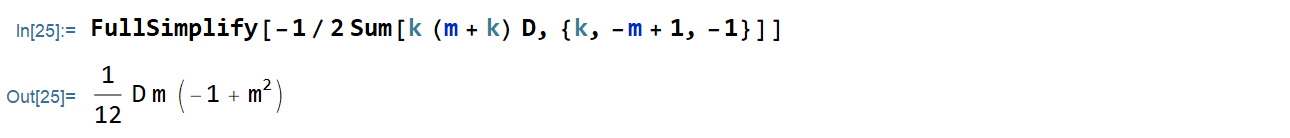
\includegraphics[width=14cm]{cap.PNG}
\end{figure}
Comparing this result to \eqref{eq:algebra}, we see that $c=D$. The only case we having treated yet is for $m<1$, but since $[L_m,L_{-m}]=-[L_{-m},L_{m}]$ the result just obtained holds here as well.
\section*{Problem 2}
We have to show explicitly that
\begin{equation} \label{eq:jacobi}
	\{[Q_B,L_m],b_n\}-\{[L_m,b_n],Q_B\}-[\{b_n,Q_B\},L_m]=0
\end{equation}
For later convenience we will list the following (anti-)commutators found in Polchinski
\begin{equation}
	\begin{aligned}
		\{Q_B,b_m\}&=L_m^m+L_m^g=L_m\\
		\{Q_B,Q_B\}&=0\\
		[L_m,L_n]&=(m-n)L_{m+n}+\frac{c}{12}(m^3-m)\delta_{(m+n)\,0}\\
		[L_m,\mathcal{O}_n]&=[(h-1)m-n]\mathcal{O}_{m+n}
	\end{aligned}
\end{equation}
where $h$ in the last line is the weight $(h,0)$ of the corresponding tensor $\mathcal{O}(z)$. In the case of $b(z)$ which has weight $(2,0)$ this is
\begin{equation}
	\begin{aligned}
		[L_m,b_n]&=(m-n)b_{m+n}
	\end{aligned}
\end{equation}
Looking at each term of \eqref{eq:jacobi} one by one 
\begin{equation}
	\begin{aligned}
		\{[L_m,b_n],Q_B\}=&\{L_mb_n,Q_B\}-\{b_nL_m,Q_B\}\\
		=&L_mb_nQ_B+Q_BL_mb_n-b_nL_mQ_B-Q_Bb_nL_m\\
		[\{b_n,Q_B\},L_m]=&[b_nQ_B,L_m]+[Q_Bb_n,L_m]\\
		=&b_nQ_BL_m-L_mb_nQ_B+Q_Bb_nL_m-L_mQ_Bb_n\\
		\{[Q_B,L_m],b_n\}=&\{Q_BL_m,b_n\}-\{L_mQ_B,b_n\}\\
		=&Q_BL_mb_n+b_nQ_BL_m-L_mQ_Bb_n-b_nL_mQ_B\\
	\end{aligned}
\end{equation}
Summing these according to \eqref{eq:jacobi}, they all cancel as expected
\begin{equation}
	\begin{aligned}
		&-L_mb_nQ_B-Q_BL_mb_n+b_nL_mQ_B+Q_Bb_nL_m\\
		&-b_nQ_BL_m+L_mb_nQ_B-Q_Bb_nL_m+L_mQ_Bb_n\\
		&+Q_BL_mb_n+b_nQ_BL_m-L_mQ_Bb_n-b_nL_mQ_B\\
		&=0
	\end{aligned}
\end{equation}
Using the Jacobi identity we can then show
\begin{equation}
	\begin{aligned}
		\{[Q_B,L_m],b_n\}&=[\{b_n,Q_B\},L_m]+\{[L_m,b_n],Q_B\}\\
		=&-\{L_m,L_n\}+(m-n)\{b_{n+m},Q_b\}=-\{L_m,L_n\}+(m-n)L_m\\
		=&-\frac{c}{12}(m^3-m)\delta_{m+n\, 0}\\
	\end{aligned}
\end{equation}
which is zero for $c=0$. As noted by Polchinski, this implies that the commutator $[Q_B,L_m]=0$. Lastly, taking the following version of  the Jacobi identity for $Q_BQ_Bb_n$
\begin{equation}
	[\{X,Y\},Z]=-[\{Y,Z\},X]-[\{Z,X\},Y]
\end{equation}
We have:
\begin{equation}
	\begin{aligned}
		2[Q_B^2,b_n] =&
		[\{Q_B,Q_B\},b_n]=[\{Q_B,b_n\},Q_B]-[\{b_n,Q_B\},Q_B]=2[L_m,Q_B]
	\end{aligned}
\end{equation}
Again, we expect this to be zero for $c=0$ and contain no c-ghost modes. Since it does in fact have a ghost number this, just as in the previous case, implies that $Q_B^2=0$. 
\section*{Problem 3}
Here we will use the gauge boson vertex operator
\begin{equation}
    \frac{-ig_0}{\sqrt{2\alpha'}}\epsilon_\mu :\dot{X}^\mu e^{ik\cdot X}:
\end{equation}
With the exponential OPE's
\begin{equation}
\expval{\prod_{i=1}^n:e^{ik_i\ \cdot X(y_i)}:}_{D_2}=(2\pi)^D\delta^D\left(\sum_ik_i\right)\prod_{i<j}|y_{ij}|^{2\alpha' k_i\cdot k_j}
\end{equation}
In general we have the OPE
\begin{equation} \label{eq:ope}
\begin{aligned}
&\expval{\prod_{i=1}^n:e^{ik_i\ \cdot X(y_i)}:\prod_{j=1}^p\partial_y X^{\mu_j}(y_j')}_{D_2}\\
&=iC_{D_2}^X(2\pi)^D\delta^D\left(\sum_ik_i\right)\prod_{i<j}|y_{ij}|^{2\alpha' k_i\cdot k_j}\expval{\prod_{j=1}^p\left[v^{\mu_j}(y_j')+q^{\mu_j}(y_j')\right]}
\end{aligned}
\end{equation}
with the $q$'s being contracted using $-2\alpha'\frac{\eta^{\mu\nu}}{(y-y')^{2}}$ and 
\begin{equation}\label{eq:vmom}
    v^{\mu}(y)=-2i\alpha'\sum_{i=1}^n\frac{k_i^\mu}{y-y_i}
\end{equation}
Before proceeding we will only consider one of the cyclic orderings and gauge-fix. Taking the ordering in figure fig 6.2e from Polchinski, see Figure \ref{fig:1}, we may fix the points $y_1,\,y_2,\,$ and $y_3$. The fact that the circle jumps from $-\infty $ to $\infty$ at the point 3 and that the arrow shows the direction of increase, indicates that $-\infty< y_1< y_3 < y_2<\infty $, so that we can gauge fix $y_1=0,\,y_2=\infty$, and $y_3=1$
\begin{figure}[htb!]
    \centering
    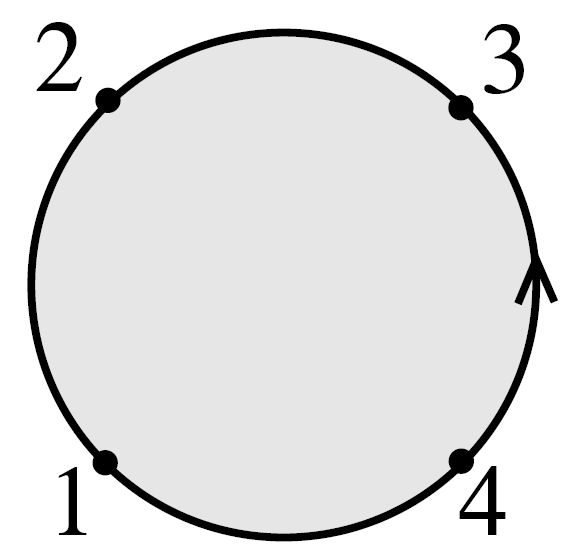
\includegraphics[width=4cm]{E.png}
    \caption{Ordering from Polchinski}
    \label{fig:1}
\end{figure}
This ordering has the following contribution in terms of the gauge boson vertex operators and the Chan-Paton factors
\begin{equation}\label{eq:int}
e^{-\lambda}\frac{g_0^4}{4\alpha'^2}\int \dd y_4\expval{:\epsilon_3\cdot \dot{X} e^{ik_3\cdot X(y_3)}::\epsilon_4\cdot \dot{X} e^{ik_4\cdot X(y_4)}::\epsilon_1\cdot \dot{X} e^{ik_1\cdot X(y_1)}::\epsilon_2\cdot \dot{X} e^{ik_2\cdot X(y_2)}:}_{D_2}\Tr(\lambda^{a_3a_2a_1a_4})
\end{equation}
where the integration domain of $y_4$ can be seen from the figure as well. The OPE \ref{eq:ope} specializes in $D=26$ and for $n=4$ to
\begin{equation}
\begin{aligned}
&\expval{\prod_{i=1}^4: \epsilon_i \cdot \dot X e^{ik_i\ \cdot X(y_i)}:}_{D_2}\\
=&i(2\pi)^{26}C_{D_2}^X C_{D_2}^g\delta^{26}\left(\sum_ik_i\right)\left(|y_{12}|^{2\alpha' k_1\cdot k_2}|y_{13}|^{2\alpha' k_1\cdot k_2}|y_{14}|^{2\alpha' k_1\cdot k_4}|y_{23}|^{2\alpha' k_2\cdot k_3}|y_{24}|^{2\alpha' k_2\cdot k_4}|y_{34}|^{2\alpha' k_3\cdot k_4}\right)\\
&\times\epsilon_{1\,\mu_1}\epsilon_{2\,\mu_2}\epsilon_{3\,\mu_3}\epsilon_{4\,\mu_4}\expval{\left[v^{\mu_1}(y_1)+q^{\mu_1}(y_1)\right]\left[v^{\mu_2}(y_2)+q^{\mu_2}(y_2)\right]\left[v^{\mu_3}(y_3)+q^{\mu_3}(y_3)\right]\left[v^{\mu_4}(y_4)+q^{\mu_4}(y_4)\right]}
\end{aligned}
\end{equation}
recalling from equation \eqref{eq:vmom} that the $v$'s are all function of the momenta and since the problem states to find the part of the amplitude proportional to $(\epsilon_1\cdot \epsilon_2)(\epsilon_3\cdot \epsilon_4)$ we may ignore them.
\begin{equation}
\begin{aligned}
=&i(2\pi)^{26}\delta^{26}C_{D_2}^X C_{D_2}^g\left(\sum_ik_i\right)\left(|y_{12}|^{2\alpha' k_1\cdot k_2}|y_{13}|^{2\alpha' k_1\cdot k_2}|y_{14}|^{2\alpha' k_1\cdot k_4}|y_{23}|^{2\alpha' k_2\cdot k_3}|y_{24}|^{2\alpha' k_2\cdot k_4}|y_{34}|^{2\alpha' k_3\cdot k_4}\right)\\
&\times\epsilon_{1\,\mu_1}\epsilon_{2\,\mu_2}\epsilon_{3\,\mu_3}\epsilon_{4\,\mu_4}\expval{q^{\mu_1}(y_1)q^{\mu_2}(y_2)q^{\mu_3}(y_3)q^{\mu_4}(y_4)}
\end{aligned}
\end{equation}
As explained underneath Pol Vol 1 eq (6.2.20) the expectation value of the $q(y_i)$'s are just all ways of contracting $-2\alpha'\frac{\eta^{\mu\nu}}{(y_i-y_j')^{2}}$. Since we are looking for a specific polarization contraction, we can once again pick out a specific contribution
\begin{equation}\label{eq:some}
\begin{aligned}
=&i(2\pi)^{26}C_{D_2}^X C_{D_2}^g\delta^{26}\left(\sum_ik_i\right)\left(|y_{12}|^{2\alpha' k_1\cdot k_2}|y_{13}|^{2\alpha' k_1\cdot k_2}|y_{14}|^{2\alpha' k_1\cdot k_4}|y_{23}|^{2\alpha' k_2\cdot k_3}|y_{24}|^{2\alpha' k_2\cdot k_4}|y_{34}|^{2\alpha' k_3\cdot k_4}\right)\\
&\times(\epsilon_{1}\cdot \epsilon_{2})(\epsilon_{3}\cdot \epsilon_{4})\frac{4\alpha'^2}{y_{12}^2y_{34}^2}
\end{aligned}
\end{equation}
Then using
\begin{equation}
C_{D_2}^X C^{g}_{D_2}e^{-\lambda }=\frac{1}{\alpha' g_0^2}
\end{equation}
We find inserting \eqref{eq:some} into \eqref{eq:int} 
\begin{equation} \label{eq:genform}
\begin{aligned}
&i\frac{g_0^2}{\alpha'}(2\pi)^{26}\delta^{26}\left(\sum_ik_i\right)(\epsilon_{1}\cdot \epsilon_{2})(\epsilon_{3}\cdot \epsilon_{4})
|y_{12}|^{2\alpha' k_1\cdot k_2+1}|y_{13}|^{2\alpha' k_1\cdot k_3+1}|y_{23}|^{2\alpha' k_2\cdot k_3+1}\frac{1}{y_{12}^2}\\
&\times \Tr(\lambda^{a_3}\lambda^{a_2}\lambda^{a_1}\lambda^{a_4})\,\int_{y_1}^{y_3} \dd y_4\:|y_{14}|^{2\alpha' k_1\cdot k_4}|y_{24}|^{2\alpha' k_2\cdot k_4}|y_{34}|^{2\alpha' k_3\cdot k_4} \frac{1}{y_{34}^2}
\end{aligned}
\end{equation}
Employing the gauge-fixing discussed in the beginning: $y_1=0,\,y_2=\infty$, and $y_3=1$
\begin{equation}
\begin{aligned}
y_{12}&=|y_1-y_2|\sim y_2\\
y_{13}&=|y_1-y_3|= 1\\
y_{14}&=|y_1-y_4|=y_4\\
y_{23}&=|y_2-y_3|\sim y_2\\
y_{24}&=|y_2-y_4|\sim y_2\\
y_{34}&=|y_3-y_4|=\underbrace{|1-y_4|=1-y_4}_{0<y_4<1}\\
\end{aligned}
\end{equation}
Inserting these
\begin{equation}
\begin{aligned}
&i\frac{g_0^2}{\alpha'}(2\pi)^{26}\delta^{26}\left(\sum_ik_i\right)(\epsilon_{1}\cdot \epsilon_{2})(\epsilon_{3}\cdot \epsilon_{4})
|y_{2}|^{2\alpha' k_1\cdot k_2-1+2\alpha'k_2\cdot k_3+1+2\alpha' k_2\cdot k_4}\\
&\times \Tr(\lambda^{a_3}\lambda^{a_2}\lambda^{a_1}\lambda^{a_4})\,\int_{y_1}^{y_3} \dd y_4\:(1-y_4)^{2\alpha' k_1\cdot k_4}|y_{4}|^{2\alpha' k_3\cdot k_4-2}\\
=&
i\frac{g_0^2}{\alpha'}(2\pi)^{26}\delta^{26}\left(\sum_ik_i\right)(\epsilon_{1}\cdot \epsilon_{2})(\epsilon_{3}\cdot \epsilon_{4})\Tr(\lambda^{a_1}\lambda^{a_4}\lambda^{a_3}\lambda^{a_2})\,\int_{0}^{1} \dd y_4\:(1-y_4)^{-\alpha' u}y_{4}^{-\alpha's-2}\\
\end{aligned}
\end{equation}
where we have set $u=-2k_1\cdot k_3$ and $s=-2k_1\cdot k_2$. The last integral is just the beta function. The remaining six orderings contributing can now be found through appropriate permutations of the $\lambda$'s and $k$'s. We will start from equation \eqref{eq:genform} since the gauge choice is where the differences show up in the calculation. Writing $\kappa\equiv i\frac{g_0^2}{\alpha'}(2\pi)^{26}\delta^{26}\left(\sum_ik_i\right)(\epsilon_{1}\cdot \epsilon_{2})(\epsilon_{3}\cdot \epsilon_{4})$ and taking each ordering from fig. 6.2 in Polchinski, we find for each one
\\\\
\underline{\textbf{(1,2,3,4):}}\\
Gaugefix: $y_1=1,\,y_2=\infty$, and $y_3=0$
\begin{equation}
\begin{aligned}
\kappa \Tr(\lambda^{a_1}\lambda^{a_2}\lambda^{a_3}\lambda^{a_4})\,\int_{0}^{1} \dd y_4\:(1-y_4)^{\alpha' u}y_{4}^{-\alpha's-2}
\end{aligned}
\end{equation}
\\\\
\underline{\textbf{(1,4,2,3):}}\\
Gaugefix: $y_1=0,\,y_2=1$, and $y_3=\infty$
\begin{equation}
	\begin{aligned}
		\kappa \Tr(\lambda^{a_1}\lambda^{a_4}\lambda^{a_2}\lambda^{a_3})\,\int_{0}^{1} \dd y_4\:(1-y_4)^{\alpha' t}y_{4}^{-\alpha'u}
	\end{aligned}
\end{equation}
\\\\
\underline{\textbf{(1,2,4,3):}}\\
Gaugefix: $y_1=\infty,\,y_2=0$, and $y_3=1$
\begin{equation}
	\begin{aligned}
		\kappa \Tr(\lambda^{a_1}\lambda^{a_2}\lambda^{a_4}\lambda^{a_3})\,\int_{0}^{1} \dd y_4\:(1-y_4)^{\alpha' t}y_{4}^{-\alpha's-2}
	\end{aligned}
\end{equation}
\\\\
\underline{\textbf{(1,3,2,4):}}\\
Gaugefix: $y_1=1,\,y_2=0$, and $y_3=\infty$
\begin{equation}
\begin{aligned}
\kappa \Tr(\lambda^{a_1}\lambda^{a_3}\lambda^{a_2}\lambda^{a_4})\,\int_{0}^{1} \dd y_4\:(1-y_4)^{\alpha' t}y_{4}^{-\alpha'u}
\end{aligned}
\end{equation}
\\\\
\underline{\textbf{(1,3,4,2):}}\\
Gaugefix: $y_1=\infty,\,y_2=1$, and $y_3=0$
\begin{equation}
	\begin{aligned}
		\kappa \Tr(\lambda^{a_1}\lambda^{a_3}\lambda^{a_4}\lambda^{a_2})\,\int_{0}^{1} \dd y_4\:(1-y_4)^{\alpha' t}y_{4}^{-\alpha's-2}
	\end{aligned}
\end{equation}
\\\\
Summing all six orderings
\begin{equation}
\begin{aligned}
A_4=\kappa& \left[\Tr(\lambda^{a_1}\lambda^{a_2}\lambda^{a_3}\lambda^{a_4})+\Tr(\lambda^{a_1}\lambda^{a_4}\lambda^{a_3}\lambda^{a_2})\right]\,\int_{0}^{1} \dd y_4\:(1-y_4)^{\alpha' u}y_{4}^{-\alpha's-2}\\
&\times\left[\Tr(\lambda^{a_1}\lambda^{a_4}\lambda^{a_2}\lambda^{a_3})+\Tr(\lambda^{a_1}\lambda^{a_3}\lambda^{a_2}\lambda^{a_4})\right]\,\int_{0}^{1} \dd y_4\:(1-y_4)^{\alpha' t}y_{4}^{-\alpha'u}\\
&\times\left[\Tr(\lambda^{a_1}\lambda^{a_2}\lambda^{a_4}\lambda^{a_3})+\Tr(\lambda^{a_1}\lambda^{a_3}\lambda^{a_4}\lambda^{a_2})\right]\,\int_{0}^{1} \dd y_4\:(1-y_4)^{\alpha' t}y_{4}^{-\alpha's-2}
\end{aligned}
\end{equation}
The beta-functions can be approximated for $\alpha'\to 0$ with
\begin{figure}[H]
    \centering
    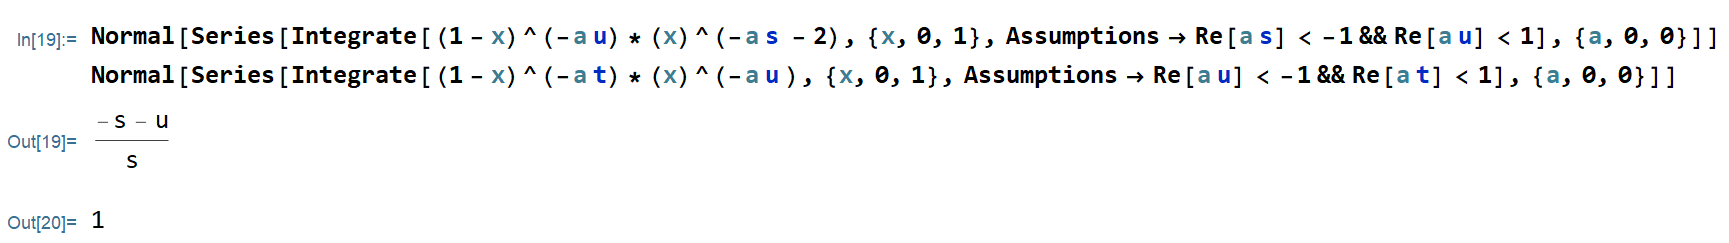
\includegraphics[width=18cm]{cal.png}
\end{figure}
So that by setting the Yang-Mills coupling $g_{\text{YM}}=\frac{g_0}{\sqrt{\alpha'}}$ we find
\begin{equation} \label{eq:STYM}
	\begin{aligned}
ig_{\text{YM}}^2(2\pi)^{26}\delta^{26}\left(\sum_ik_i\right)(\epsilon_{1}\cdot \epsilon_{2})(\epsilon_{3}\cdot \epsilon_{4})& \left[\Tr(\lambda^{a_1}\lambda^{a_2}\lambda^{a_3}\lambda^{a_4})+\Tr(\lambda^{a_1}\lambda^{a_4}\lambda^{a_3}\lambda^{a_2})\right]\,(-1-\frac{u}{s})\\
&\times\left[\Tr(\lambda^{a_1}\lambda^{a_4}\lambda^{a_2}\lambda^{a_3})+\Tr(\lambda^{a_1}\lambda^{a_3}\lambda^{a_2}\lambda^{a_4})\right]\\
&\times\left[\Tr(\lambda^{a_1}\lambda^{a_2}\lambda^{a_4}\lambda^{a_3})+\Tr(\lambda^{a_1}\lambda^{a_3}\lambda^{a_4}\lambda^{a_2})\right]\,(-1-\frac{u}{t})
\end{aligned}
\end{equation}
The YM amplitude from Feynman diagrams is easily found, using Feynman rules and here we will just reuse one of our old calculations from which we have found that the terms contributing to $(\epsilon_1\cdot\epsilon_2)(\epsilon_3\cdot\epsilon_4)$ comes from only the contact diagram and the $s$-channel \footnote{Neglecting factors of $2\pi$ and the delta-function. Everything is in Feynman gauge.}
\begin{align*}
	i\mathcal{A}_c=&-ig_{\text{YM}}^2\\
	&\times\lp[f^{abc}f^{cde}\lp((\epsilon_1\cdot \epsilon_4)(\epsilon_2\cdot\epsilon_3)-(\epsilon_1\cdot \epsilon_3)(\epsilon_2\cdot \epsilon_4)\rp)\rp.\\
	&\phantom{\times[}\lp.+f^{ace}f^{bde}\lp((\epsilon_1\cdot \epsilon_2)(\epsilon_4\cdot\epsilon_3)-(\epsilon_1\cdot \epsilon_3)(\epsilon_2\cdot \epsilon_4)\rp)\rp]\\
	&\phantom{\times[}\lp.+f^{ade}f^{bce}\lp((\epsilon_1\cdot \epsilon_2)(\epsilon_4\cdot\epsilon_3)-(\epsilon_1\cdot \epsilon_4)(\epsilon_2\cdot \epsilon_3)\rp)\rp]\\
\end{align*}
\begin{align*}
	i\mathcal{A}_s
	=&-\frac{ig_{\text{YM}}^2}{s}f^{abe}f^{ecd}\\
	&\times \lp[\lp(2p_1\cdot \epsilon_2\rp)\epsilon_1^\alpha - (2p_2\cdot \epsilon_1)\epsilon_2^\alpha+(p_2-p_1)^\alpha (\epsilon_1\cdot \epsilon_2)\rp]\\
	&\times\lp[(p_4-p_3)_\alpha (\epsilon_3\cdot\epsilon_4) + (2p_3\cdot \epsilon_4)\epsilon_{3\,\alpha}-(2p_4\cdot\epsilon_3)\epsilon_{4,\,\alpha}\rp]\\
\end{align*}
so taking the terms we are looking for we find 
\begin{equation} \label{eq:YM}
\begin{aligned}
-ig_{\text{YM}}^2(\epsilon_1\cdot \epsilon_2)(\epsilon_4\cdot\epsilon_3)\left[
f^{ace}f^{bde}+f^{ade}f^{bce}+\frac{u-t}{s}f^{abe}f^{ecd}\right]
\end{aligned}
\end{equation}
using the identity\footnote{This identity holds for both U$(N)$ and SU$(N)$}
\begin{equation}
	f^{abe}f^{cde}=-\frac{1}{2}\Tr([\lambda^a,\lambda^b][\lambda^c,\lambda^d])
\end{equation}
the $f^{abc}$ can then be expanded in terms of traces and the Yang-Mills amplitude \eqref{eq:YM} matches the $\alpha\to0$ limit of the string amplitude \eqref{eq:STYM} after insertion of the delta functions and factors of $2\pi$:
\end{document}
